\documentclass[11pt]{article}
\usepackage[a4paper,margin=2.2cm]{geometry}
\usepackage[T1]{fontenc}
\usepackage{lmodern}
\usepackage{booktabs}
\usepackage{amsmath}
\usepackage{graphicx}
\usepackage{xcolor}
\usepackage{tikz}
\usetikzlibrary{positioning,arrows.meta}
\usepackage[hidelinks]{hyperref}
\usepackage{caption}
\captionsetup{font=small,labelfont=bf}
\usepackage{float}
\usepackage{enumitem}
\setlist{nosep}

\definecolor{accent}{HTML}{1a7f6e}
\definecolor{panel}{HTML}{f3f5f7}
\newcommand{\code}[1]{\texttt{\small #1}}

% ---- FireSVM benchmark numbers (filled from reports/waveshare_fire_results.json)
\newcommand{\fireacc}{96.4\%}
\newcommand{\fireprec}{99.7\%}
\newcommand{\firerec}{75.5\%}
\newcommand{\firefone}{85.9\%}
\newcommand{\firefar}{0.04\%}
\newcommand{\firetp}{314}\newcommand{\firetn}{2410}
\newcommand{\firefp}{1}\newcommand{\firefn}{102}
\newcommand{\firetrain}{6{,}497}\newcommand{\firetest}{2{,}827}
\newcommand{\firetestpos}{416}

\title{\bfseries Production Checkpoint Report\\
\large FireSVM \,\textperiodcentered\, MobileNet-SSD \,\textperiodcentered\, Thermo-X3D~T5v2\\
\normalsize Smart Thermal System for Patient Safety Monitoring}
\author{Guy Chen \and Yaniv Blau \and Roy Lieberman\\
\small Supervisor: Or Zilberberg \quad Advisor: Dr.\ Oshrit Hoffer \quad Afeka College of Engineering}
\date{July 4, 2026}

\begin{document}
\maketitle

\begin{abstract}
\noindent This report documents the three model checkpoints deployed in the live
demonstration system: the \textbf{FireSVM} fire detector, the
\textbf{MobileNet-SSD} person detector, and the \textbf{Thermo-X3D~T5v2}
contact (touch) detector. For each model we describe the architecture,
inputs and outputs, feature extraction, loss and optimizer, the heuristics
that surround the network, benchmark accuracy
(accuracy/precision/recall/F$_1$/FAR), and measured CPU runtime with
estimates for the Raspberry~Pi~5 target. All sensing is thermal-only
(Waveshare 80$\times$62 module, 8\,Hz) --- no optical imagery is ever captured.
\end{abstract}

\section{System context}

Three thermal cameras observe the room. Each 8\,Hz tick produces three raw
$62\times80$ frames in $^\circ$C. Two preprocessing views feed the models
(an empirically-validated split --- see \S\ref{sec:x3d-configd}):

\begin{itemize}
\item \textbf{Raw frames} go to the per-camera detectors (FireSVM,
      MobileNet-SSD). Raw input transfers across rooms without recalibration.
\item \textbf{Tateno residuals} (Gaussian smooth $\rightarrow$ background
      subtract $\rightarrow$ rectified $L_1$ residual) against a
      \emph{session-local rolling 25th-percentile background} go to
      Thermo-X3D. The p25 background is computed from the last $\sim$30\,s
      of frames and refreshed continuously --- no per-room calibration,
      $\sim$2\,s warm-up.
\end{itemize}

\begin{table}[H]\centering\small
\begin{tabular}{lllr}
\toprule
Task & Checkpoint file & Format & Size\\
\midrule
Fire      & \code{fire\_svm\_detector/\_default.thalg} & sklearn pickle & 64\,KB\\
Person    & \code{mobilenet\_ssd\_detector/Waveshare\_26984\_raw.onnx} & ONNX & 0.27\,MB\\
Contact   & \code{thermo\_x3d\_detector/Waveshare\_26984\_T5\_v2.ftz.onnx} (+meta) & ONNX & 1.6\,MB\\
\bottomrule
\end{tabular}
\caption{Deployed checkpoints. All are committed on the \code{demo-linux}
branch; total $\approx$2\,MB. The two neural networks run via
\code{onnxruntime} --- the deployment is torch-free.}
\end{table}

\section{FireSVM --- fire detection}

\subsection{What is an SVM?}

A support vector machine is a binary classifier that finds the separating
hyperplane $w^\top\phi(x)+b=0$ with the \emph{maximum margin} --- the largest
distance to the nearest training points of either class. Only those nearest
points (the \emph{support vectors}) determine the boundary, which makes the
model compact and robust. Two extensions make SVMs practical:

\begin{itemize}
\item \textbf{Soft margin ($C$).} Real classes overlap, so slack variables
      allow some points inside the margin; $C$ trades margin width against
      training violations ($C{=}1$ here).
\item \textbf{Kernel trick.} Instead of computing $\phi(x)$ explicitly, a
      kernel $k(x,x')=\langle\phi(x),\phi(x')\rangle$ evaluates inner
      products in a high-dimensional space. We use the radial basis
      function kernel
      $k(x,x') = \exp(-\gamma\|x-x'\|^2)$ with
      $\gamma=\text{scale}=1/(d\cdot\mathrm{Var}(X))$, which yields a
      smooth non-linear decision boundary.
\end{itemize}

Prediction is $\hat y=\mathrm{sign}\!\left(\sum_i \alpha_i y_i\,
k(x_i,x)+b\right)$ over the support vectors $x_i$. A logistic fit on the
decision values (\emph{Platt scaling}) turns the raw margin into the
confidence probability we report.

\subsection{What is special about our FireSVM}

FireSVM is not applied to pixels. A classical segmentation stage proposes a
region, and the SVM classifies six scalar statistics of that region --- which
makes the model \emph{resolution-invariant} (the same checkpoint works on
32$\times$24 and 80$\times$62 sensors) and extremely fast.

\paragraph{Pipeline (per raw frame).}
\begin{enumerate}
\item \textbf{Region proposal --- Otsu segmentation.} The frame is
      histogrammed (256 bins); Otsu's criterion selects the threshold
      maximizing between-class variance; the binary mask is shaped by one
      $3{\times}3$ erosion and two dilations.
\item \textbf{Feature extraction.} Connected components are extracted and
      the \emph{hottest blob} is selected. Six features describe it:
      $\max$ temperature, mean, standard deviation, area, skewness and
      kurtosis of the blob's pixel distribution. (Fire blobs are small,
      extremely hot and heavy-tailed; people are large, near 36$^\circ$C
      and symmetric.)
\item \textbf{Standardization.} Features are $z$-scored with the
      $\mu,\sigma$ learned at fit time.
\item \textbf{Classification.} RBF-SVC ($C{=}1$, $\gamma{=}$scale, 874
      support vectors) outputs SAFE or ACTIVE\_COM\-BUS\-TION with a
      Platt confidence.
\end{enumerate}

\paragraph{Input/output.} In: one raw $62\times80$ float32 frame
($^\circ$C). Out: a \code{FireAlert} --- level, Platt confidence, and the
hottest blob's features including its bounding box (drawn in the demo UI).

\paragraph{Training.} Frames with a YOLO class-0 (fire) box are positives;
all other labeled frames are SAFE. Stratified sequential 70/30 split per
(scene, camera, class). No gradient training --- the SVC solves its convex
dual (SMO); there is no optimizer/epoch schedule, and regularization is the
$C$ soft margin.

\paragraph{Runtime note.} Profiling showed 88\% of inference time was
\emph{scipy call overhead} for skewness/kurtosis ($\sim$13 blobs $\times$ 2
calls per frame). Replacing them with an algebraically identical numpy
implementation (verified bit-identical on 1{,}395 real blobs) cut predict
from 8.8 to \textbf{1.19\,ms/frame} with zero behavioral change.

\begin{table}[H]\centering\small
\begin{tabular}{lccccc|cccc}
\toprule
& Accuracy & Precision & Recall & F$_1$ & FAR & TP & TN & FP & FN\\
\midrule
FireSVM (test) & \fireacc & \fireprec & \firerec & \firefone & \firefar
& \firetp & \firetn & \firefp & \firefn\\
\bottomrule
\end{tabular}
\caption{FireSVM benchmark --- \firetest{} held-out test frames
(\firetestpos{} fire-positive) from the 70/30 protocol;
\firetrain{} training frames. FAR is the false-alarm rate over
fire-free frames. The near-zero FAR is the design priority for a ward:
the detector essentially never cries wolf, at the cost of missing
low-contrast ignition frames (small cigarette embers at distance).}
\end{table}

\section{MobileNet-SSD --- person detection}

\subsection{Architecture}

A single-stage anchor-based detector (SSD) on a MobileNet-style backbone,
sized for our tiny native input --- we do \emph{not} upscale the thermal
frame to 300$\times$300 like standard SSD; the network runs on
$1\times62\times80$ directly. The backbone is built from
\textbf{depthwise-separable convolutions} (depthwise $3{\times}3$ + pointwise
$1{\times}1$, each with BatchNorm+ReLU), the MobileNet trick that cuts
multiply--accumulates roughly 8--9$\times$ versus dense convolutions.

\begin{table}[H]\centering\small
\begin{tabular}{llll}
\toprule
Stage & Operator & Stride & Output ($C\times H\times W$)\\
\midrule
Input &  &  & $1\times62\times80$\\
Stem & Conv $3{\times}3$ + BN + ReLU & 2 & $16\times31\times40$\\
Block 1 & DW-separable & 1 & $32\times31\times40$\\
Block 2 & DW-separable & 2 & $64\times15\times20$ \; ($\rightarrow$ \textbf{F1})\\
Block 3 & DW-separable & 1 & $64\times15\times20$\\
Block 4 & DW-separable & 2 & $128\times7\times10$ \; ($\rightarrow$ \textbf{F2})\\
Block 5 & DW-separable & 1 & $128\times7\times10$\\
\midrule
Head (F1) & Conv $3{\times}3$ $\rightarrow$ $K(4{+}2)$ ch & 1 & box $12\times15\times20$, cls $6\times15\times20$\\
Head (F2) & Conv $3{\times}3$ $\rightarrow$ $K(4{+}2)$ ch & 1 & box $12\times7\times10$, cls $6\times7\times10$\\
\bottomrule
\end{tabular}
\caption{MicroMobileNet-SSD, Waveshare configuration. Two detection
scales: F1 (fine, near people) and F2 (coarse, large/close people).
$K{=}3$ anchors per cell $\Rightarrow$ $15{\cdot}20{\cdot}3 +
7{\cdot}10{\cdot}3 = 1110$ anchors total.}
\end{table}

\begin{figure}[h]\centering
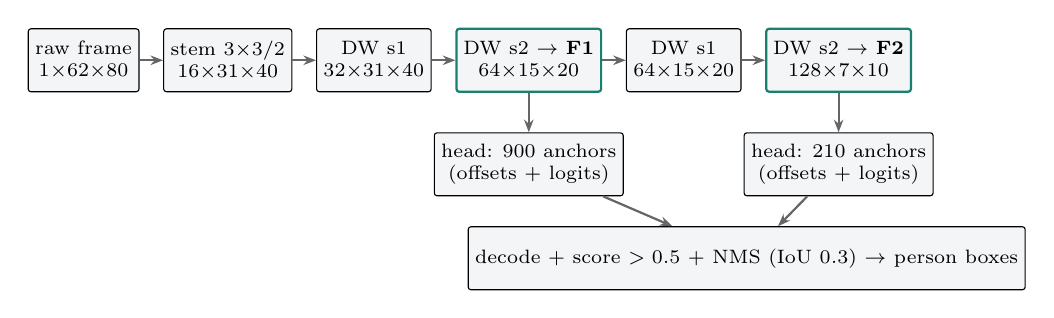
\begin{tikzpicture}[
  node distance=3mm,
  blk/.style={draw, rounded corners=1pt, fill=panel, minimum height=8mm,
              inner sep=2.5pt, font=\scriptsize, align=center},
  arr/.style={-{Stealth[length=1.6mm]}, thick, draw=black!60}]
\node[blk] (in) {raw frame\\ $1{\times}62{\times}80$};
\node[blk, right=of in] (stem) {stem $3{\times}3$/2\\ $16{\times}31{\times}40$};
\node[blk, right=of stem] (b1) {DW s1\\ $32{\times}31{\times}40$};
\node[blk, right=of b1, draw=accent, thick] (f1) {DW s2 $\to$ \textbf{F1}\\ $64{\times}15{\times}20$};
\node[blk, right=of f1] (b3) {DW s1\\ $64{\times}15{\times}20$};
\node[blk, right=of b3, draw=accent, thick] (f2) {DW s2 $\to$ \textbf{F2}\\ $128{\times}7{\times}10$};
\node[blk, below=5mm of f1] (h1) {head: 900 anchors\\ (offsets + logits)};
\node[blk, below=5mm of f2] (h2) {head: 210 anchors\\ (offsets + logits)};
\node[blk, below=17mm of b3, xshift=8mm] (dec) {decode + score $>0.5$ + NMS (IoU $0.3$) $\to$ person boxes};
\draw[arr] (in) -- (stem);
\draw[arr] (stem) -- (b1);
\draw[arr] (b1) -- (f1);
\draw[arr] (f1) -- (b3);
\draw[arr] (b3) -- (f2);
\draw[arr] (f1) -- (h1);
\draw[arr] (f2) -- (h2);
\draw[arr] (h1) -- (dec);
\draw[arr] (h2) -- (dec);
\end{tikzpicture}
\caption{Data flow. (Block 5, a stride-1 refinement after F2, omitted for clarity.)}
\end{figure}

\paragraph{Anchors.} Each feature-map cell holds $K{=}3$ anchor boxes with
aspect ratios $\{1{:}1,\;1{:}2,\;1{:}3\}$ (square, tall, very tall ---
person-shaped) and base widths of 10\,px (F1) and 16\,px (F2) in input
coordinates.

\paragraph{Input/output.} In: one raw frame, per-frame $z$-scored
($x\!-\!\mu)/(\sigma\!+\!10^{-6})$. Out: for each of the 1110 anchors, 4 box
offsets and 2 class logits. Offsets are decoded against the anchor
($cx,cy$ scaled by variance 0.1; $w,h$ by $e^{0.2\,d}$), softmax scores are
thresholded at 0.5, and greedy non-maximum suppression (IoU $0.3$) yields
the final \code{(x,y,w,h,score)} person boxes.

\subsection{Loss, optimizer, heuristics}

\textbf{Loss} is the standard SSD multi-task objective. Anchors are matched
to ground truth by IoU (positive $\geq0.5$, negative $<0.4$, in-between
ignored):
\[
\mathcal{L} \;=\; \frac{1}{N_{pos}}\Big(
\underbrace{\textstyle\sum \mathrm{CE}(\text{cls})}_{\text{pos + hard negatives}}
\;+\; \lambda \underbrace{\textstyle\sum \mathrm{SmoothL1}(\text{loc})}_{\text{positives only}}
\Big), \qquad \lambda = 1.
\]
\textbf{Hard-negative mining} keeps only the 3 highest-loss background
anchors per positive (3:1), preventing the 1110-to-few anchor imbalance
from drowning the signal. \textbf{Optimizer:} Adam, lr $10^{-3}$, weight
decay $10^{-4}$ (the only explicit regularizer besides BatchNorm), 50
epochs. \textbf{Augmentation:} random horizontal flips and small random
translations (zero-padded), boxes transformed accordingly.

\subsection{Results}

Benchmarked on the Waveshare dataset with an 80/10/10 timeline split
(frame-level presence; box quality as mean IoU of matched detections):

\begin{table}[H]\centering\small
\begin{tabular}{lcccccc}
\toprule
Detector (test) & Accuracy & Precision & Recall & F$_1$ & FAR & mean IoU\\
\midrule
AdaptiveThreshold & 76.6\% & 93.4\% & 80.7\% & 86.6\% & 83.0\% & 0.565\\
HOG+SVM           & 79.8\% & 92.7\% & 85.1\% & 88.7\% & 98.1\% & 0.585\\
\textbf{MobileNet-SSD} & \textbf{95.8\%} & \textbf{99.1\%} & \textbf{96.4\%} & \textbf{97.7\%} & \textbf{13.2\%} & \textbf{0.673}\\
\bottomrule
\end{tabular}
\caption{Person detection, 825 test frames (772 with people). FAR is
computed over the 53 person-free test frames (7 false alarms). The deployed
checkpoint is the \emph{raw-input} variant of the same architecture and
training recipe: a preprocessing ablation showed the SSD performs best on
raw frames (and transfers across rooms), while background-subtracted
residuals belong to the contact model.}
\end{table}

\noindent For deployment the network was exported to ONNX with the
anchor decode and NMS re-implemented in numpy; parity vs.\ the PyTorch path
was verified at $7.6\times10^{-6}$ max box/score difference over 330 boxes.

\section{Thermo-X3D T5v2 --- contact (touch) detection}

\subsection{Architecture}

Contact between people is a \emph{spatio-temporal} event --- two warm blobs
approaching, merging, and interacting over seconds. Thermo-X3D is a small
video CNN inspired by the X3D family: it processes a sliding window of
$T{=}5$ consecutive residual frames from all three cameras and outputs one
contact probability. It is \emph{pixel-based end-to-end}: no bounding
boxes, no cross-camera geometry, and crucially \textbf{no homography or
per-room calibration} (a hard product constraint --- 800 rooms).

Every convolution is \textbf{(2+1)D-factorized}: a spatial $1{\times}3{\times}3$
kernel followed by a temporal $3{\times}1{\times}1$ kernel. Factorization
halves parameters and FLOPs versus full $3^3$ kernels, doubles the
non-linearities, and --- practically --- means every op is effectively a 2-D
convolution, which CPU inference libraries optimize well.

\begin{table}[H]\centering\small
\begin{tabular}{llll}
\toprule
Stage & Operator & Spatial stride & Output ($C\times T\times H\times W$)\\
\midrule
Input (per camera) & & & $1\times5\times62\times80$\\
Stem & Conv $1{\times}3{\times}3$ + BN + ReLU & 1 & $24\times5\times62\times80$\\
ResBlock 1 & (2+1)D + attention + skip & 1 & $24\times5\times62\times80$\\
ResBlock 2 & (2+1)D + attention + skip & 2 & $48\times5\times31\times40$\\
ResBlock 3 & (2+1)D + attention + skip & 2 & $96\times5\times16\times20$\\
Pool + proj & global avg pool, Linear $96{\to}128$ & & $128$\\
\midrule
Fusion & concat 3 camera streams & & $384$\\
Head & Linear $384{\to}64$, ReLU, Linear $64{\to}2$ & & $2$ logits\\
\bottomrule
\end{tabular}
\caption{Thermo-X3D T5v2. Three \emph{independent} per-camera encoder
streams (late fusion). 382{,}562 parameters total.}
\end{table}

Each residual block is: spatial conv $\rightarrow$ BN/ReLU $\rightarrow$
temporal conv $\rightarrow$ BN/ReLU $\rightarrow$ \textbf{thermal attention}
$\rightarrow$ add skip ($1{\times}1{\times}1$ conv when shape changes)
$\rightarrow$ ReLU. The attention module is CBAM-style, adapted to thermal
statistics where \emph{maxima} matter (hot spots):

\begin{itemize}
\item \emph{Channel attention:} global average- \textbf{and} max-pool over
      $(T,H,W)$, each through a shared 2-layer MLP (reduction 4), summed,
      sigmoid-gated per channel.
\item \emph{Spatial attention:} channel-wise mean and max maps concatenated,
      convolved $1{\times}7{\times}7$, sigmoid-gated per location.
\end{itemize}

\begin{figure}[h]\centering
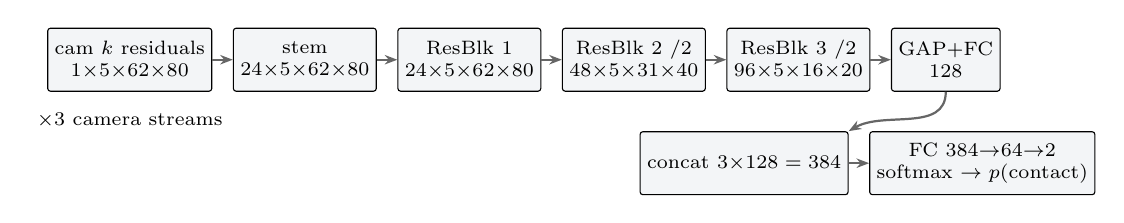
\begin{tikzpicture}[
  node distance=2.6mm,
  blk/.style={draw, rounded corners=1pt, fill=panel, minimum height=8mm,
              inner sep=2.5pt, font=\scriptsize, align=center},
  arr/.style={-{Stealth[length=1.6mm]}, thick, draw=black!60}]
\node[blk] (in) {cam $k$ residuals\\ $1{\times}5{\times}62{\times}80$};
\node[blk, right=of in] (stem) {stem\\ $24{\times}5{\times}62{\times}80$};
\node[blk, right=of stem] (b1) {ResBlk 1\\ $24{\times}5{\times}62{\times}80$};
\node[blk, right=of b1] (b2) {ResBlk 2 /2\\ $48{\times}5{\times}31{\times}40$};
\node[blk, right=of b2] (b3) {ResBlk 3 /2\\ $96{\times}5{\times}16{\times}20$};
\node[blk, right=of b3] (gp) {GAP+FC\\ $128$};
\draw[arr] (in) -- (stem); \draw[arr] (stem) -- (b1);
\draw[arr] (b1) -- (b2); \draw[arr] (b2) -- (b3); \draw[arr] (b3) -- (gp);
\node[blk, below=5mm of b2, xshift=14mm] (cat) {concat $3{\times}128 = 384$};
\node[blk, right=of cat] (head) {FC $384{\to}64{\to}2$\\ softmax $\to p(\text{contact})$};
\draw[arr] (gp.south) to[out=-90,in=30] (cat.east|-cat.north);
\node[font=\scriptsize, below=0.5mm of in, yshift=-1mm] (x3) {$\times$3 camera streams};
\draw[arr] (cat) -- (head);
\end{tikzpicture}
\caption{One of three per-camera streams; features fuse late.}
\end{figure}

\paragraph{Inputs/outputs.} In: for each camera, the Tateno residual
against the rolling p25 background, globally $z$-scored
($\mu{=}0.868$, $\sigma{=}0.786$, statistics of the training pixels); a
rolling buffer holds the last $T{=}5$ frames per camera, so each 8\,Hz tick
re-evaluates the network on a $(3,5,62,80)$ volume spanning 0.625\,s. Out:
softmax contact probability. \textbf{Decision heuristics:} alarm threshold
$0.35$ (selected by validation sweep), evaluated every tick; the pipeline
supports $N$-frame persistence (deployed as benchmarked: $N{=}1$).

\subsection{Loss, optimizer, training data}

\textbf{Loss:} cross-entropy with \emph{inverse-frequency class weights}
(positives are $\sim$35\% of frames; weights $n/(2n_{neg}), n/(2n_{pos})$).
\textbf{Optimizer:} Adam, lr $10^{-3}$, weight decay $10^{-4}$, 10 epochs,
batch 8, over all $T$-frame windows of contiguous training runs.
\textbf{Data:} 57 scenes / 30{,}279 frames / 10{,}516 positive --- the home
recordings (re-annotated after a label audit) plus the 06-30 ward-archive
segments; per-scene timeline split 60/15/25; the human-labeled
\code{2men\_clash} scene is excluded entirely as a held-out benchmark.
Training uses the same p25-background residuals as deployment (v2's key fix
--- the model trains on exactly what it sees at runtime).

\subsection{Results}

\begin{table}[H]\centering\small
\begin{tabular}{lccccc}
\toprule
& Accuracy & Precision & Recall & F$_1$ & FAR\\
\midrule
In-domain test (7{,}592 frames, th $0.35$) & 91.3\% & 85.6\% & 90.1\% & 87.8\% & 8.0\%\\
Held-out \code{2men\_clash}, frame-exact & --- & 23.1\% & 62.2\% & 33.7\% & 54.4\%\\
Held-out \code{2men\_clash}, $\pm2$ frames & --- & 28.1\% & 73.7\% & 40.7\% & 51.3\%\\
\bottomrule
\end{tabular}
\caption{Thermo-X3D T5v2. The held-out gap is a \emph{label-granularity}
artifact, not pure model error: much of the training corpus carries
episode-level interval labels (contact marked continuously over
multi-minute episodes), teaching episode semantics that frame-exact
scoring penalizes. At the \emph{episode} level the model detects
5/5 contact episodes in the held-out scene with 12.8\,s of total
false-positive time. Frame-exact tightening is the main open item for
the next retrain (interval-core training or threshold recalibration).}
\end{table}

\paragraph{ONNX backend verification.} The deployed ONNX checkpoint was
re-scored on the full protocol: fp32 ONNX reproduces PyTorch \emph{exactly}
(F$_1$ 87.8\% / 33.7\%). An int8-quantized variant was also produced
(test F$_1$ 86.6\%, FAR 8.0$\to$5.2\%) but is \emph{slower} than fp32 on
x86 (no optimized int8 3-D conv path in onnxruntime) and is kept only as a
Pi-side candidate for future testing.

\subsection{The classical alternative --- ``config-D'' rule}
\label{sec:x3d-configd}

Alongside the network we maintained a hand-crafted contact rule, the best
of a long ablation series (\textbf{config-D}): run MobileNet-SSD on
\emph{raw} frames; segment warm blobs on the Tateno \emph{residual}; fire
when \emph{exactly two} person boxes fall inside one connected warm
component (the two-body merge test --- rejects person+object and 3-person
crowds); then clean the per-frame decision stream with temporal
morphological opening (2) and closing (7). This ablation also produced the
raw/residual preprocessing split now used system-wide.

On clean labels config-D and Thermo-X3D are nearly tied in-domain
(F$_1{\pm}2$: 76.9\% vs.\ 78.5\%), but on the held-out room the network won
decisively (73.1\% vs.\ 45.3\% for the earlier T5 checkpoint) --- the rule's
blob-area constants are room-tuned, which conflicts with the no-calibration
constraint. Config-D therefore remains a validation baseline; the deployed
detector is the network.

\section{Runtime}

Measured on the development PC (Intel i7-11700K class, 8 cores; single
inference, real frames). Pi~5 estimates scale the thread-matched
measurements by the per-core gap (Cortex-A76 2.4\,GHz vs.\ $\sim$4.9\,GHz;
factor $\approx$3--3.5$\times$), pending on-device validation.

\begin{table}[H]\centering\small
\begin{tabular}{lrrr}
\toprule
Model (per frame / per window) & PC CPU & PC (4 threads) & Pi 5 estimate\\
\midrule
Tateno preprocessing & 0.02\,ms & --- & $\sim$0.1\,ms\\
FireSVM & 1.19\,ms & --- & 3.5--5\,ms\\
MobileNet-SSD & 2.6\,ms & 1.8\,ms & 8--10\,ms\\
Thermo-X3D (torch fp32, before work) & 93.7\,ms & --- & ---\\
Thermo-X3D (ONNX fp32) & 34.5\,ms & --- & ---\\
\textbf{Thermo-X3D (ONNX fp32, denormals flushed)} & \textbf{12.9\,ms} & 14.7\,ms & \textbf{45--60\,ms (4 cores)}\\
Thermo-X3D (ONNX int8) & 60.8\,ms & --- & untested\\
\midrule
Full tick: $3\times$(pre+fire+person) + contact & $\approx$24\,ms & & $\approx$65--90\,ms\\
8\,Hz budget & 125\,ms & & 125\,ms\\
\bottomrule
\end{tabular}
\caption{CPU inference runtime. The X3D speedup chain is 7.3$\times$
total: ONNX export (2.7$\times$, bit-identical F$_1$), then flushing
\emph{denormal weights} --- 19.3\% of the trained weights were subnormal
floats ($\sim$10$^{-41}$, a weight-decay artifact) that trigger CPU
microcode penalties; zeroing them in the model changed no output bit
(max $|\Delta\text{logit}|=0$) and gave another 2.7$\times$. Future
retrains should clamp subnormal weights post-training.}
\end{table}

In the demo application the three per-camera stacks run on parallel worker
threads and X3D on a fourth, with depth-1 queues that drop stale frames;
the estimated Pi tick ($\sim$65--90\,ms) fits the 125\,ms budget at 8\,Hz
with margin. All numbers await confirmation on the Pi itself; the
benchmark scripts run there unmodified.

\section{Reproducibility}

\begin{itemize}
\item Benchmarks: \code{scripts/eval\_waveshare\_fire.py},
      \code{eval\_waveshare\_human.py}, \code{eval\_x3d\_backends.py},
      \code{benchmark\_inference\_cpu.py}, \code{profile\_fire\_svm.py}.
\item Result files (\code{reports/}): \code{waveshare\_fire\_results.json},
      \code{waveshare\_human\_results.json},\\
      \code{x3d\_T5\_v2\_results.json},
      \code{x3d\_backend\_comparison.json},
      \code{cpu\_inference\_benchmark.json},\\
      \code{x3d\_onnx\_runtime.json}.
\item Deployment: branch \code{demo-linux} (weights included);
      live demo \code{python -m demo.app --live}.
\end{itemize}

\end{document}
